\chapter{Señales analógicas de salida en Arduino (PWM)}

En este apartado vamos a ver los fundamentos en los que se basa la generación de salidas analógicas en Arduino. El procedimiento para generar una señal analógica es el llamado PWM.
Señal PWM (Pulse-width modulation) señal de modulación por ancho de pulso.\\
Donde:\\
\begin{itemize}
\item PW (Pulse Width) o ancho de pulso, representa al ancho (en tiempo) del pulso.
\item length/period (periodo), o ciclo , es el tiempo total que dura la señal.
\end{itemize}
La frecuencia se define como la cantidad de pulsos (estado on/off)por segundo y su expresión matemática es la inversa del periodo, como muestra la siguiente ecuación.
\begin{equation}
Frequency = \frac{1}{period}	
\end{equation}
El periodo se mide en segundos, de este modo la unidad en la cual se mide la frecuencia (hertz) es la inversa a la unidad de tiempo (segundos).\\
Existe otro parámetro asociado o que define a la señal PWM, denominado "Duty cycle", Ciclo de Trabajo, el cual determina el porcentaje de tiempo que el pulso (o voltaje aplicado) está en estado activo (on) durante un ciclo.\\
Por ejemplo, si una señal tiene un periodo de 10 ms y sus pulsos son de ancho (PW) 2ms, dicha señal tiene un ciclo de trabajo (duty cycle) de 20\% (20\% on y 80\% off). El siguiente gráfico muestra tres señales PWM con diferentes "duty cycles".\\
\begin{figure}[!htp]
	\centering
	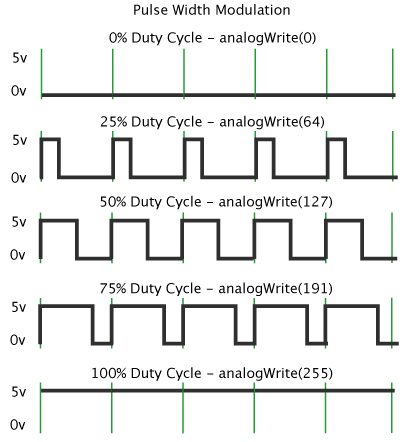
\includegraphics[width=150pt]{./Imagenes/Documentos/ArduinoNotebook_img10.png}
	\caption[ancho de pulso de modulación]{Ancho de pulo}
\end{figure}

La señal PWM se utiliza como técnica para controlar circuitos analógicos. El periodo y el ciclo de trabajo (duty cycle) del tren de pulsos puede determinar la tensión entregada a dicho circuito. Si, por ejemplo, tenemos un voltaje de 5v y lo modulamos con un duty cycle del 10\%, obtenemos 0.5V de señal analógica de salida.\\
Las señales PWM son comúnmente usadas para el control de velocidad de motores DC (si decrementas el ciclo de trabajo sobre la señal de control del circuito de potencia que actúa sobre el motor el motor se mueve más lentamente), ajustar la intensidad de brillo de un LED, etc.\\
En Arduino, con ATmega168 o ATmega328, la señal de salida PWM (pines 3,5,6,9,10, y 11) es una señal de frecuencia 490 Hz aproximadamente y que sólo nos permite cambiar el "duty cycle" o el tiempo que el pulso está activo (on) o inactivo (off), utilizando la función analogWrite().\\
Otra forma de generar señales PWM es utilizando la capacidad del microprocesador. La señal de salida obtenida de un microprocesador es una señal digital de 0 voltios (LOW) y de 5 voltios (HIGH).\\
Con el siguiente código y con sólo realizar modificaciones en los intervalos de tiempo que el pin seleccionado tenga valor HIGH o LOW, a través de la función digitalWrite (), generamos la señal PWM.
\begin{lstlisting}
/* senal PWM */

int digPin = 10; // pin digital 10

void setup() 
{
   pinMode(digPin, OUTPUT);     // pin en modo salida

}

void loop() {
   digitalWrite(digPin, HIGH); // asigna el valor HIGH al pin 
   delay(500);     // espera medio segundo
   digitalWrite(digPin, LOW); // asigna el valor LOW al pin
   delay(500);     // espera medio segundo
}
\end{lstlisting}
El programa pone el pin 10 a HIGH una vez por segundo durante medio segundo (ciclo de trabajo 50\%), la frecuencia que se genera en dicho pin es de 1 pulso por segundo o 1 Hz de frecuencia (periodo de 1 segundo). Cambiando la temporización del programa, podremos cambiar el ciclo de trabajo de la señal. Por ejemplo, si cambiamos las dos líneas con delay(500) por delay(250) y delay(750), modificamos el ciclo de trabajo a 25\%; ahora, el programa pone el pin 10 a HIGH una vez por segundo durante 1/4 de segundo y la frecuencia sigue siendo de 1 Hz.\\
Utilizando la función analogWrite(pin,value) podemos obtener la misma señal a una frecuencia de 490 Hz aproximadamente. Para una señal PWM con ciclo de trabajo 50\% hay que poner en el parámetro value, de la función analogWrite(pin,value), el valor de 127.\\
\begin{lstlisting}
/* senal PWM en el pin 10 de ciclo de trabajo 50*/

int digPin = 10; // pin digital 10

void setup() 
{
                // no se declara el modo del pin 
                //como salida analogica
}

void loop() {
   analogWrite(digPin,127); // Senal PWM a 50% en el PIN 10
}
\end{lstlisting}
\newpage{}
De forma que cambiando el valor del parámetro value en la función analogWrite(pin,value), podemos obtener distintos ciclos de trabajo:
\begin{table}[!hpt]
	\centering
	\begin{tabular}{|c|c|}
	\hline
	value & Ciclo de trabajo \\
	\hline
	0 & 0\% \\
	\hline
	63&25\%\\
	\hline
	127 & 50\% \\
	\hline
	190 & 75\% \\
	\hline
	255 & 100\%\\	
	\hline
	\end{tabular}
	\caption{Modificación de ciclos de trabajo}
\end{table}